\chapter{Binary neutron star mergers}\label{BNS-merg}

Neutron star mergers are one of the few laboratories in the universe where one can study phenomena such as gamma-ray emission, mass ejections, nucleosynthesis of heavy elements, gravitational waves, and the equation of state of supranuclear matter. For this reason,  observing events such as GW170817 and GW190425 have greatly interested the astrophysics and nuclear physics community in the last few years.
 
Numerical relativity simulations have shown how complicated the evolution of BNS systems is. Unlike the BBH case, matter effects start to play an important role in the late inspiral phase, and also in the post-merger stage. Such simulations have also shown that the evolution of the remnant object its highly dependent on  michrophysics and how high its gravitational mass with respect to the maximum mass supported by the EOS of supranuclear matter. Unfortunately, nuclear physics experiments on Earth and isolated NS observations have only taken us so far, placing some constraints on it.

Given a BNS system with known masses and spins, it has been shown that using stiff and soft EOSs within current EOS bounds may produce the following scenarios for remnant:

\begin{itemize}
\item Prompt collapse to black hole.
\item Prompt collapse to a black whole with an accretion disk.
\item Formation of a differentially rotating fluid which can be short-lived called \textit{supramassive NS} or long-lived called \textit{supramassive NS} \cite{Shibata:2019wef, Kastaun_2021}.
\end{itemize}


The following image was taken from \cite{Shibata:2019wef}. It shows how the possible outcomes listed above  can be classified by comparing the total gravitational mass of the system with the EOS-dependent threshold masses for the fast collapse $M_{thr}$(see section \ref{codeon} and \cite{Kashyap_2022}) and the maximum mass for a rigidly rotating cold NS $M_{max,spin}$.



\begin{figure}[hbt!]
\begin{center}
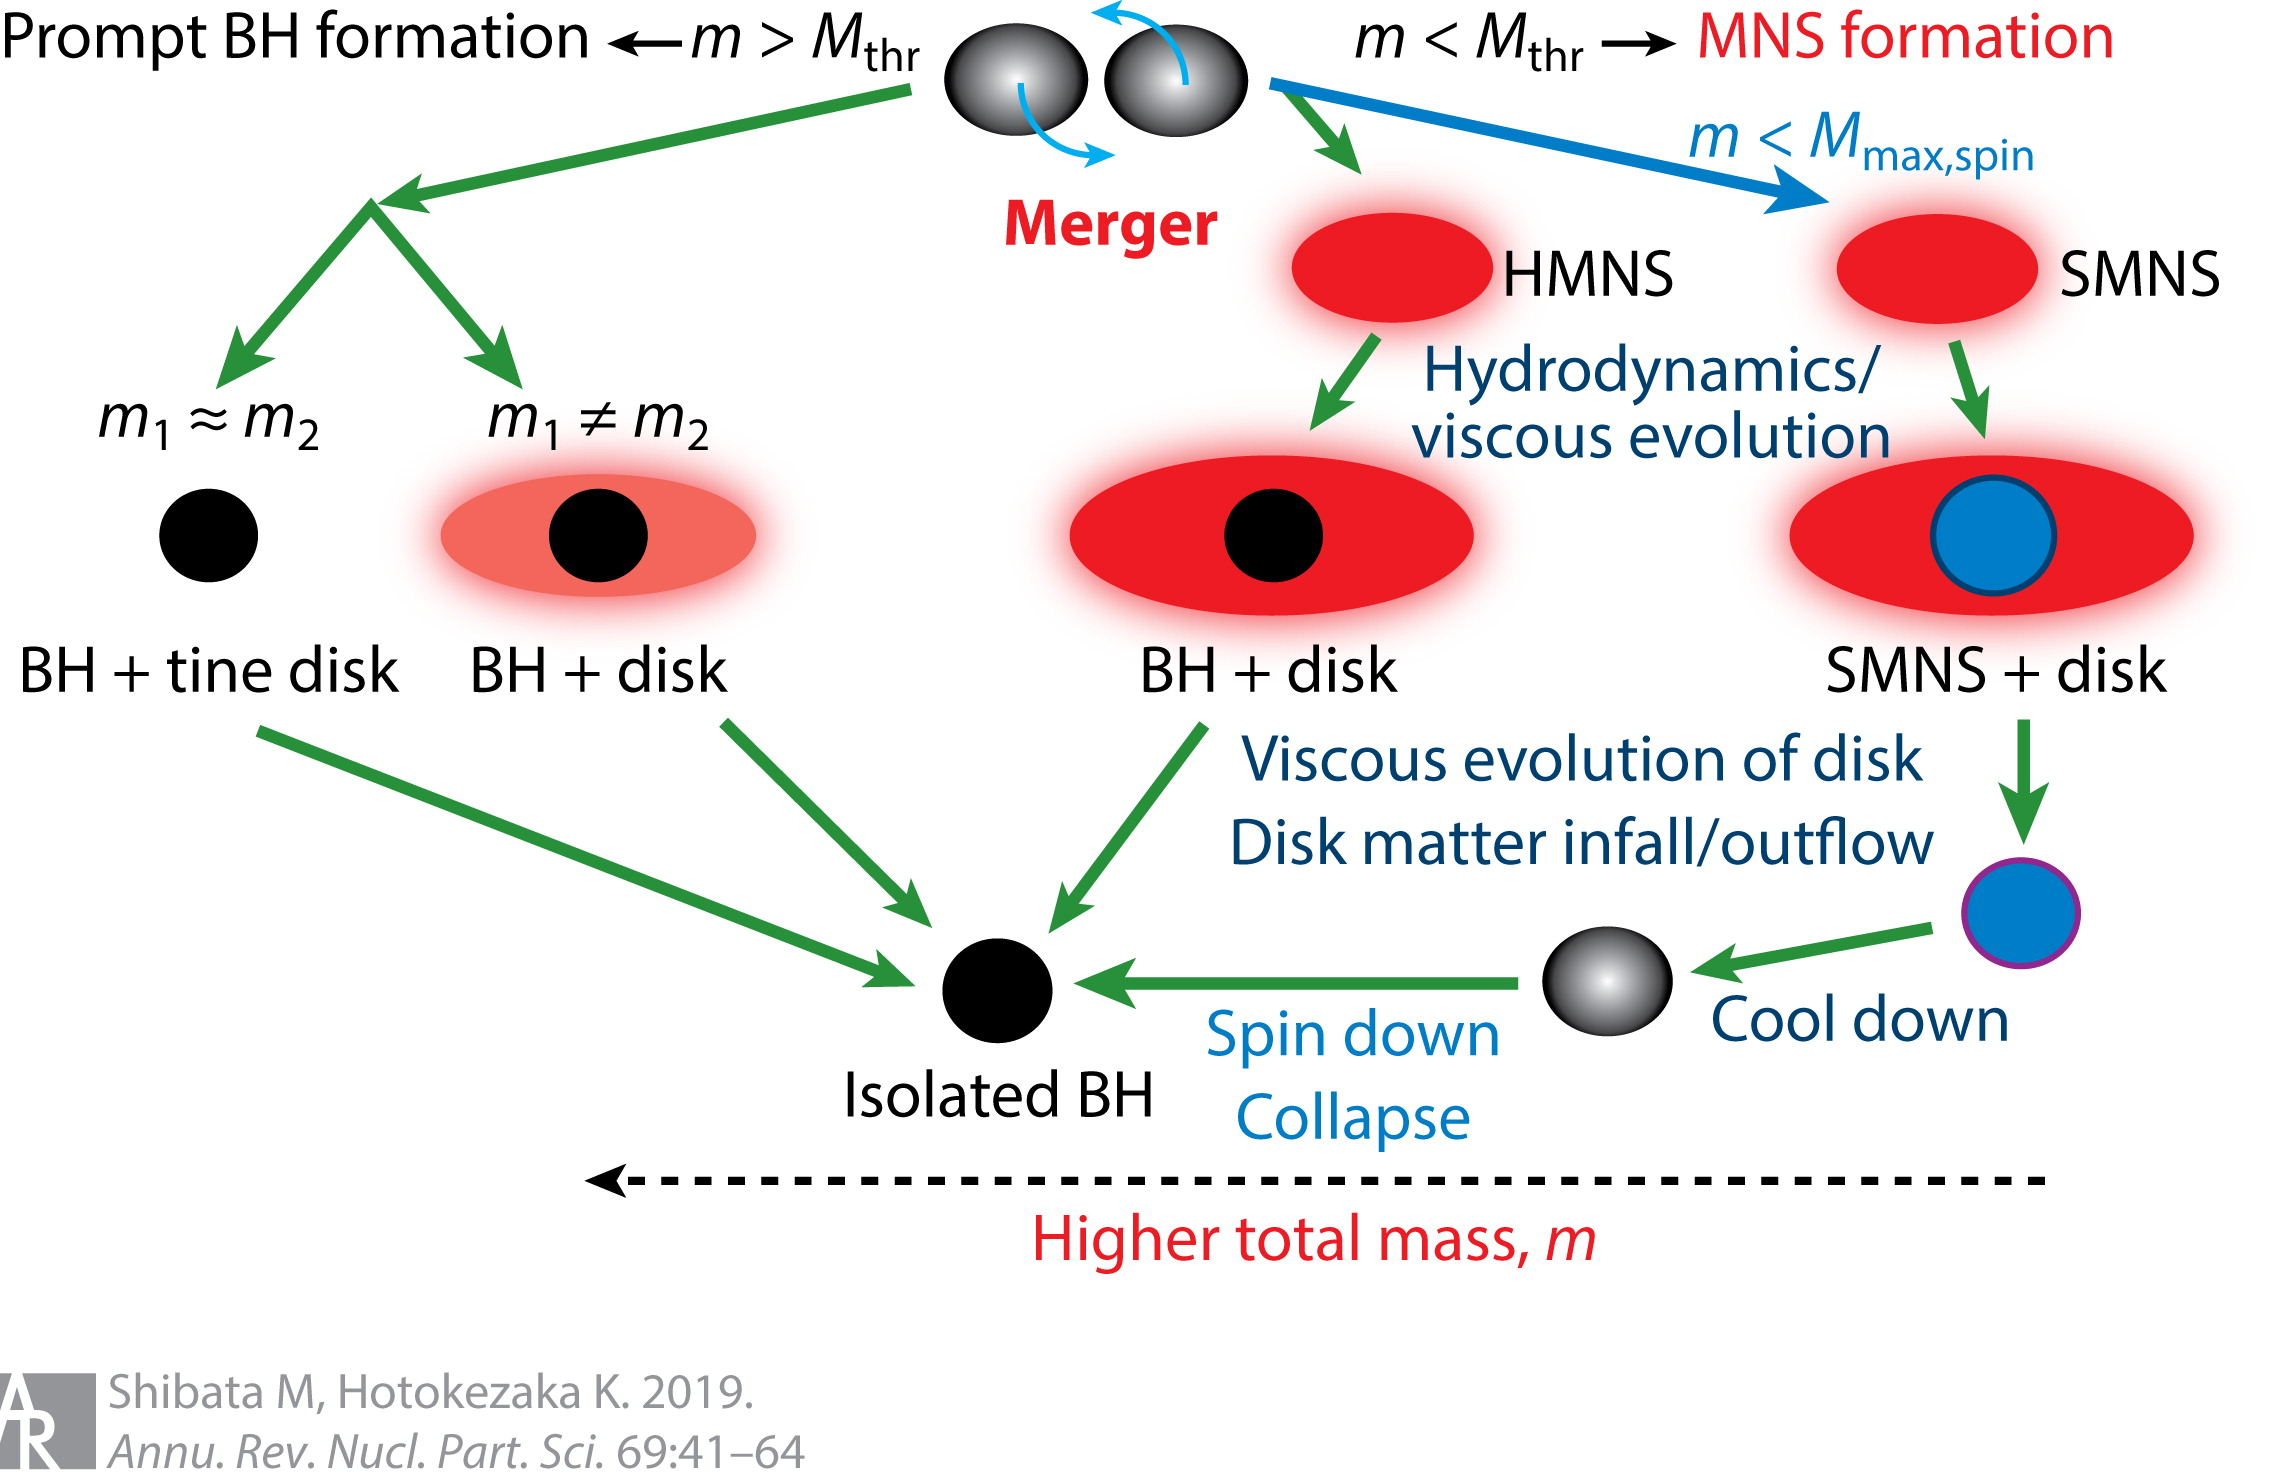
\includegraphics[width=0.5\textwidth, angle=0]{images/shi.jpeg}
\captionsetup{width=0.8\textwidth}
\caption{BNS merger remnants accoring to the EOS threshold mass}
%\caption*{This image was taken from \cite{Shibata:2019wef}. It depicts a classification of BNS postmerger remnant scenarios according to two EOS dependent parameters $M_{thr}$ and $M_{max,spin}$. Where $M_{thr}$ is the threshold masses for prompt collapse $M_{thr}$(see section \ref{codeon}) and $M_{max,spin}$ is the maximum mass for a rigidly rotating cold NS.}
\label{BNS-out}
\end{center}
\end{figure}
\FloatBarrier


The gravitational waves associated to all possible outcomes shown in figure \ref{BNS-out} will be studied in the following sections. In particular, the postmerger GWs will be extracted from a set of 200 numerical relativity BNS waveforms, and will be analized in the context of GW astronomy using simple models(see section \ref{res}).

\section{Binary neutron star waveforms}

The fact that the two body problem has no closed form solution in GR implies a big difficulty when studying the GWs generated during the evolution of compact binary systems like BBH, BNS and NSBH. For his reason, discoveries like GW150912 and GW170817 relied used theoretical models based on approximate methods like high order postnewtonian expansions, semianalitical methods like the  EOB formalism \cite{PhysRevD.96.121501,Dietrich:2018uni}  or numerical relativity simulations to study systems.


The following image is shown to depict the differences between BNS and BBH waveforms in the nonlinear regime. Notice that the BNS waveform has a complex morphology in the postmerger phase

\begin{figure}[hbt!]
\begin{center}
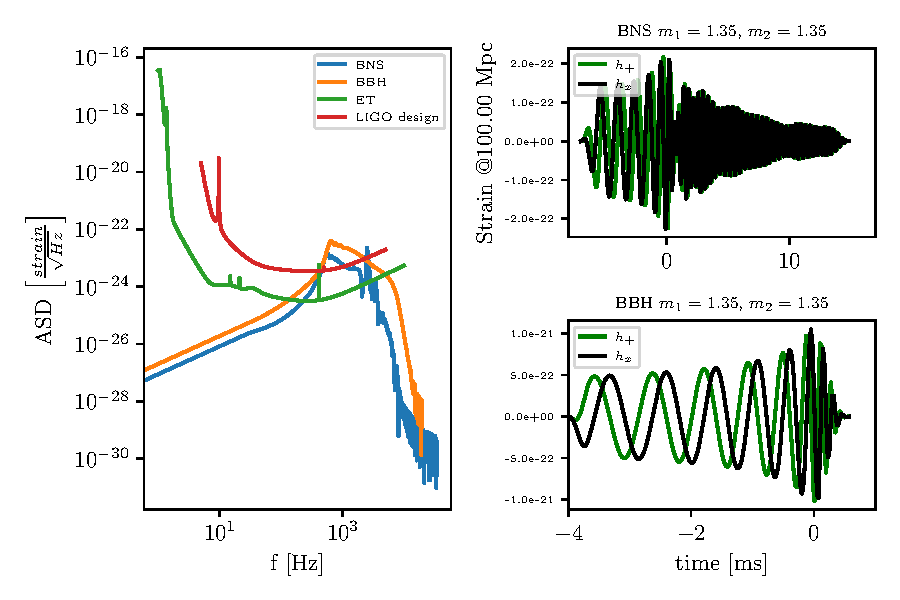
\includegraphics[width=0.6\textwidth, angle=0]{images/Data_analysis/sig_proc/BNS-BBH.pdf}
\captionsetup{width=0.8\textwidth}
\caption{Ground based detector sensitivity vs BNS and BBH signals}
\caption*{Comparison of BBH and BNS signals with same progenitor masses in the time domain(right) and frequency domain(left) at 100 MPc. Strain data was taken from \cite{Estelles:2020osj} and \cite{Dietrich:2018phi} respectively.}
\label{BBH and BNS}
\end{center}
\end{figure}

\FloatBarrier



Although aproximate and semianalitical methods like the EOB formalism \cite{Damour:2012yf,PhysRevD.96.121501,Dietrich:2018uni} have got reasonably good at reproducing the GWs until the BNS late inspiral phase, the inclusion of oscillations generated by the postmerger remnant is still state-of-the-art research. The figure below shows how numerical relativity simulations are still needed to study the entire evolution, i.e. inspiral-merger-postmerger


%the BNS waveform has a complex postmerger morphology that is hard to detect for current ground based detectors but will become relevant for third generation detectors like Einstein telescope and cosmic explorer.

\begin{figure}[hbt!]
\begin{center}

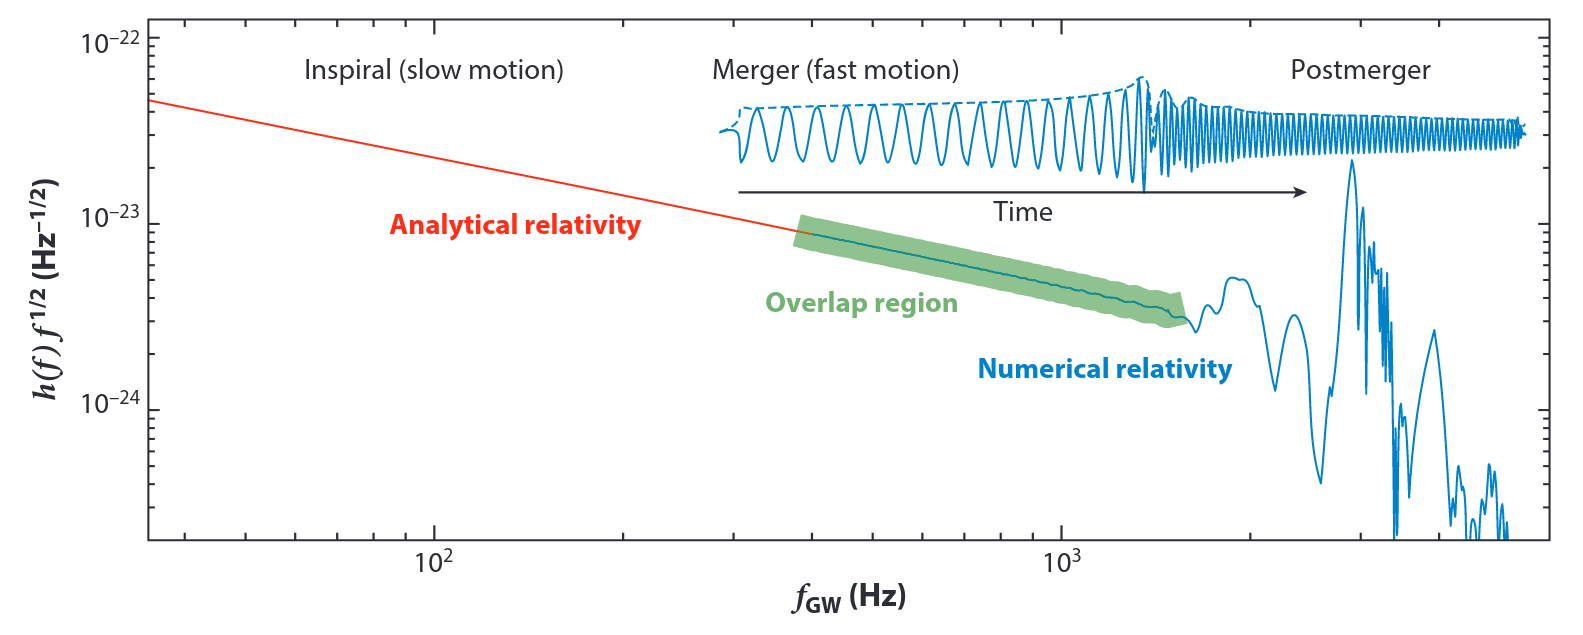
\includegraphics[width=0.65\textwidth, angle=0]{images/postmerger.png}
\captionsetup{width=0.8\textwidth}
\caption{BNS waveform: inspiral, merger and postmerger}
\caption*{This picture was taken from \cite{Radice_2020}. It shows a BNS signal and its the frequency spectrum. The waveform phases where theoretical and numerical methods are more accurate are highlighted. Notice there's an overlapping region.}
\label{BBH and BNS2}
\end{center}
\end{figure}

\FloatBarrier




The physical parameter space of BNS system can be entirely defined  in term of the masses of their constituents $m_1$ and $m_2$, their spins $\vec{S}_1$ and $\vec{S}_2$, and their tidal deformabilities $\Lambda_1$ and $\Lambda_2$\cite{Hinderer:2009ca}. However, the following derived quatities are listed below since they can be resolved much better by experiments like LIGO Virgo and KAGRA

\begin{equation}
\mathcal{M} = \frac{(m_1 m_2)^{(3/5)}}{(m_1 + m_2)^{1/5}}
\end{equation}

\begin{equation}\label{chieff}
\chi_{_{eff}} = \frac{m_1}{M}\cdot \chi_1^z + \frac{m_2}{M}\cdot \chi_2^z - \frac{38}{113} \frac{m_1 m_2}{M^2}(\chi_1^z + \chi_2^z)
\end{equation}


\begin{equation}
\tilde{\Lambda} = \frac{16}{13} \left[ \frac{(m_1 +12m_2)(m_1)^4}{M^5} \Lambda_1 + \frac{(m_2 +12m_1)(m_2)^4}{M^5} \Lambda_2 \right]
\end{equation}

where $\chi_j = \frac{S_j}{m_j}$ is the dimensionless spin parameter, and $\Lambda_j = \frac{2k_2}{3(C_j)^5}$ accounts for the dominant effect of the tidal deformability  which depends on the $l=2$ gravitoelectric love number given by

\begin{equation}
k_l = \frac{(2l-1)!}{2}\frac{G \mu_l}{R^{2l+1}}
\end{equation}

Where coeficients $\mu_l$ result from the solution of stationary perturbations of spherical relativistic stars \cite{PhysRevD.80.084035,PhysRevD.80.084018,PhysRevD.77.021502,2020GReGr..52..108B}.

The GWs can be extracted from simulations using several methods. Some extract the weyl scalar $\psi^4$ in coordinate spheres of finite radius $R$ \cite{Bishop:2016lgv,Thorne:1980ru} decompsing the radiation field in spin-weighted spherical harmonics, and others use the Cauchy characteristic method to get the radiation field at null infinity \cite{Barkett:2019uae}.

\begin{equation}\label{pso}
R\psi^4(t) = - R(\ddot{h}_+ - i\ddot{h}_\times)(t) = \sum_{l=-2}^{\infty}  \sum_{m=-l}^{l} A_{_{_{lm}}}(t) \cdot {}_{_{_{-2}}}Y_{_{_{lm}}}(\theta, \phi)
\end{equation}

Where the coefficients $A_{lm}$ are obtained by integrating the weyl scalar over the angular  part

\begin{equation}
A_{_{_{lm}}} = \oint \psi^4({}_{_{_{-2}}}Y^{*}_{_{_{lm}}}(\theta, \phi)) d\Omega
\end{equation}

We can integrate the weyl scalar to obtain the metric perturbations h decomposed in spin-weighted spherical harmonics
$ h_{lm} = - \int dt' dt'' \psi_{lm}^4$
 
\begin{equation}\label{fvr}
RH(t) = R(h_+ - ih_{\times})(t) = \sum_{l=-2}^{\infty}  \sum_{m=-l}^{l} h_{_{_{lm}}}(t) \cdot {}_{_{_{-2}}}Y_{_{_{lm}}}(\theta, \phi)
\end{equation}

\begin{mdframed}
\textbf{Remark:} keep in mind that  GW detectors observe a real valued linear combination of $h_+$ and $h_\times$ that depends on the detector angular coordinates $\theta$ and $\phi$  and the polarization angle $\psi$ (see Sathyaprakash et.al. \cite[section 4.2.1]{Sathyaprakash:2009xs})

\begin{equation}
h(t) = F^{+}(\theta, \phi, \psi) h_+(t) + F^{\times}(\theta, \phi, \psi) h_{\times}(t)
\end{equation}

\begin{equation}
\begin{aligned}
& F_{+}=\frac{1}{2}\left(1+\cos ^2 \theta\right) \cos 2 \phi \cos 2 \psi-\cos \theta \sin 2 \phi \sin 2 \psi, \\
& F_{\times}=\frac{1}{2}\left(1+\cos ^2 \theta\right) \cos 2 \phi \sin 2 \psi+\cos \theta \sin 2 \phi \cos 2 \psi
\end{aligned}
\end{equation}
\end{mdframed}


Several observables can be computed using the complex strain $H(t)$ and the complex strain components $h_{l,m}$ such as:

\begin{itemize}

\item The energy and angular momentum carried by the waves \cite{Ruiz_2007}

%\begin{equation}
%\mathcal{E}_{rad} = \lim_{r\to\infty} \frac{c^2 r^2}{16\pi G} \sum_{l=-2}^{\infty}  \sum_{m=-l}^{l} \int_{-\infty}^{t} dt'' \Biggr| \int_{-\infty}^{t''} A_{_{_{lm}}} dt' \Biggr|
%\end{equation}
%
%
%\begin{equation}
%\mathcal{J}_{z-rad} = \lim_{r\to\infty} -\frac{i \cdot c^2 r^2}{16\pi G} Im \int_{-\infty}^{t}dt'\left[ \sum_{l=-2}^{\infty} \sum_{m=-l}^{l} m  \left(\int_{-\infty}^{t'} \int_{-\infty}^{t''} dt''dt''' A_{_{_{lm}}}\right)  \cdot \left( \int_{-\infty}^{t'} dt'' (A_{_{_{lm}}})^* \right) \right]
%\end{equation}

\begin{equation}
\mathcal{E}_{rad} = \lim_{r\to\infty} \frac{c^2 r^2}{16\pi G} \sum_{l=-2}^{\infty}  \sum_{m=-l}^{l} \int_{-\infty}^{t} dt'' \Biggr|  \dot{h}_{_{_{lm}}}(t'')  \Biggr|
\end{equation}


\begin{equation}
\mathcal{J}_{z-rad} = \lim_{r\to\infty} -\frac{i \cdot c^2 r^2}{16\pi G} Im \int_{-\infty}^{t}dt'\left[ \sum_{l=-2}^{\infty} \sum_{m=-l}^{l} m  \left(h_{lm}\right)  \cdot \left( \dot{h}^*_{lm} \right) \right]
\end{equation}

\item Signal features like frequency and duration using amplitude weighted averages.

\begin{equation}\label{dwei}
d_{wei} = \frac{\int_{t_{*}}^{\infty} \left| H(t) \right| \cdot t \hspace{1mm}dt }{\int_{t_{*}}^{\infty} \left| H(t) \right| dt}
\end{equation}

\begin{equation}\label{fwei}
f_{wei} = \frac{\int_{t_{*}}^{\infty}  \left| H(t) \right| \cdot \dot{\phi}(t)  dt }{\int_{t_{*}}^{\infty} \left| H(t) \right|dt}
\end{equation}

Where $t_{*}$ its a finite time where the waveform starts, $\left| H(t) \right|$ is the strain's envelope and $\dot{\phi}(t)$ its phase velocity given by 

\begin{equation}\label{curnc}
\dot{\phi}(t)=\frac{d}{dt} \left[ \arctan \left( \frac{Im(H)}{Re(H)} \right)(t) \right]
\end{equation}

\end{itemize}



\newpage
\section{Numerical relativity waveform catalogs}\label{NR}

BNS systems have been successfully evolved on supercomputers around the world using various numerical relativity codes since the 2000s \cite{Shibata:1999hn,Shibata:1999wm,Shibata:2019wef}. Results from various authors have been collected in data sets of systems with different spins, masses, EOSs, and resolutions called NR catalogs. Unfortunately, since each simulation can take weeks on a supercomputer, mapping every point in the parameter space of a BNS to fully relativistic simulation is a task beyond the reach of current high-performance computing facilities. For example, since the intrinsic parameters of a BNS system are the tidal deformabilities, spins, masses, filling the parameter space of quasicircular BNS mergers would entail filling a discrete 6-dimensional hypercube in a sufficiently dense manner so that most regions of that space are optimally sampled. Therefore, existing catalogs are more of an unordered collection of hundreds of simulation results, rather than an attempt to sample the physical parameter space of a CBC in an optimal way. 


In particular, this thesis uses the results of two NR catalogs that sum up to about $220$ waveforms; Most of them provided by the CoRe BNS collaboration \cite{Dietrich:2018phi} which collects the results of 160 simulations covering a wide variety of studies related to neutron star physics \cite{Bernuzzi:2014kca,Dietrich:2016hky,Bernuzzi:2016pie,Dietrich:2017aum, Dietrich:2016lyp,Dietrich:2015pxa,Dietrich:2017xqb,Radice:2017zta,Bernuzzi:2014owa,Dietrich:2015iva,Bernuzzi:2015rla, Radice:2016gym,Radice:2016rys,Radice:2017lry,Dietrich:2017feu, Zappa:2017xba}, and a collection of about 60 waveforms computed by other groups for similar purposes \cite{Maione:2016zqz, Kastaun:2016elu,Maione:2017aux,Ciolfi:2017uak,Feo:2016cbs, Kawamura:2016nmk,DePietri:2015lya,DePietri:2018tpx}.

The set of 220 simulations has been run using different numerical relativity codes that evolve the Einstein equations in their 3+1 composition, such as the Einstein toolkit \cite{Loffler:2011ay,Mosta:2013gwu}, BAM \cite{PhysRevLett.92.211101,PhysRevD.77.024027,Thierfelder:2011yi}, THC \cite{Radice_2012} and Whisky \cite{Baiotti:2003btu,Giacomazzo:2007ti}, as well as codes such as LORENE \cite{lorene} and SGRID \cite{Tichy_2009,Tichy_2012,Dietrich_2015} to generate the initial conditions of the BNS system.  In the following we will briefly describe each catalog separately:


\begin{itemize}

\item CoRe BNS catalog (164 waveforms).

This catalog includes a dataset with a wide variety of BNS merger simulations with different resolutions and equations of state \cite{Banik_2014,Steiner:2012rk,PhysRevD.79.124032}. It takes into account systems with equal masses, high mass ratios, spinning binaries, and highly eccentric systems (see figure \ref{corecat}).

The simulations use LORENE or SGRID to construct the initial data. In addition, they are run using the BSSNOK \cite{PhysRevD.52.5428,1987PThPS..90....1N,Bernuzzi_2010} or Z4c \cite{Ruiz_2011,Weyhausen_2012,Hilditch_2013} formulations to evolve spacetime and matter effects via general relativistic hydrodynamics. Simulations in this catalog use two different codes: BAM and THC. Some mergers in the catalog included the effects of EOSs with microphysics and neutrino cooling, via a neutrino leakage scheme and viscous effects using the large eddy scheme GRLES \cite{Radice_2017}. It should be noted that this catalog does not include simulations with magnetic fields yet.

\item Collection of about 60 waveforms calculated by Kawamura et. al. \cite{Kawamura:2016nmk}, De Petri et.al. \cite{DePietri:2018tpx,DePietri:2015lya}, Feo et.al. \cite{Feo:2016cbs}, Kastaun et.al. \cite{Kastaun:2016elu}, Maione et.al. \cite{Maione:2016zqz,Maione:2017aux} and Ciolfi et.al. \cite{Ciolfi:2017uak}

This dataset covers smaller a subset of the BNS physical parameter(see figure \ref{lalcat}). It contains the results of around 60 simulations with different resolutions and equations of state \cite{PhysRevC.82.015806,PhysRevC.83.035802,PhysRevC.58.1804,PhysRevD.79.124032,PhysRevLett.67.2414,PhysRevC.52.2072}.

Most of these simulations used public codes like LORENE, the Einstein toolkit to evolve the binary systems.  Although most of these simulations do not take magnetic fields into account, those computed in \cite{Kawamura:2016nmk,Ciolfi:2017uak} are an exception. 

\end{itemize}



\section{The binary neutron star postmerger waveform}

Inspiral-merger-postmerger BNS GW waveform models are still under development. Most of them only cover the GW oscilations until the late inspiral phase \cite{Hinderer:2009ca,Damour:2012yf,PhysRevD.96.121501,Dietrich:2018uni}, since the merger and postmerger phase are particularly challenging to model. In recent years there has been a great interest in completing the postmerger phase such models with sophisticated phenomenological aproximants \cite{Breschi:2019srl, Tsang:2019esi, Soultanis:2021oia, https://doi.org/10.48550/arxiv.2205.09112} with the aim of using them in GW searches to improve existing EOS constraints for supranuclear matter. However, such models require a high-dimensional parameter space to reproduce the postmerger morphology, are not properly calibrated to NR waveforms across the whole parameter space nor ready to use in low latency GW search pipelines and parameter estimation runs for computational cost reasons. 

For that reason, the following description of the postmerger signal from the signal processing point of view, in the time-domain, will rely only on the sample of around 220 numerical relativity waveforms mentioned in the previous section \ref{NR}.


The complex strain \ref{fvr} of a postmerger GW signal can be described as an overmodulated complex-valued signal \cite{Kastaun:2016elu}. Such a signal may have several local amplitude minima correlated to peaks in the phase velocity \ref{curnc}.

This can also be seen in the complex plane in polar coordinates, as the orbits of $|H|(\phi)$ approach to the origin, while the orbits of $\dot{\phi}(\phi)$ reach a maximum. The figure below is intended to show such correlation in the complex plane


\begin{figure}[hbt!]
\begin{center}
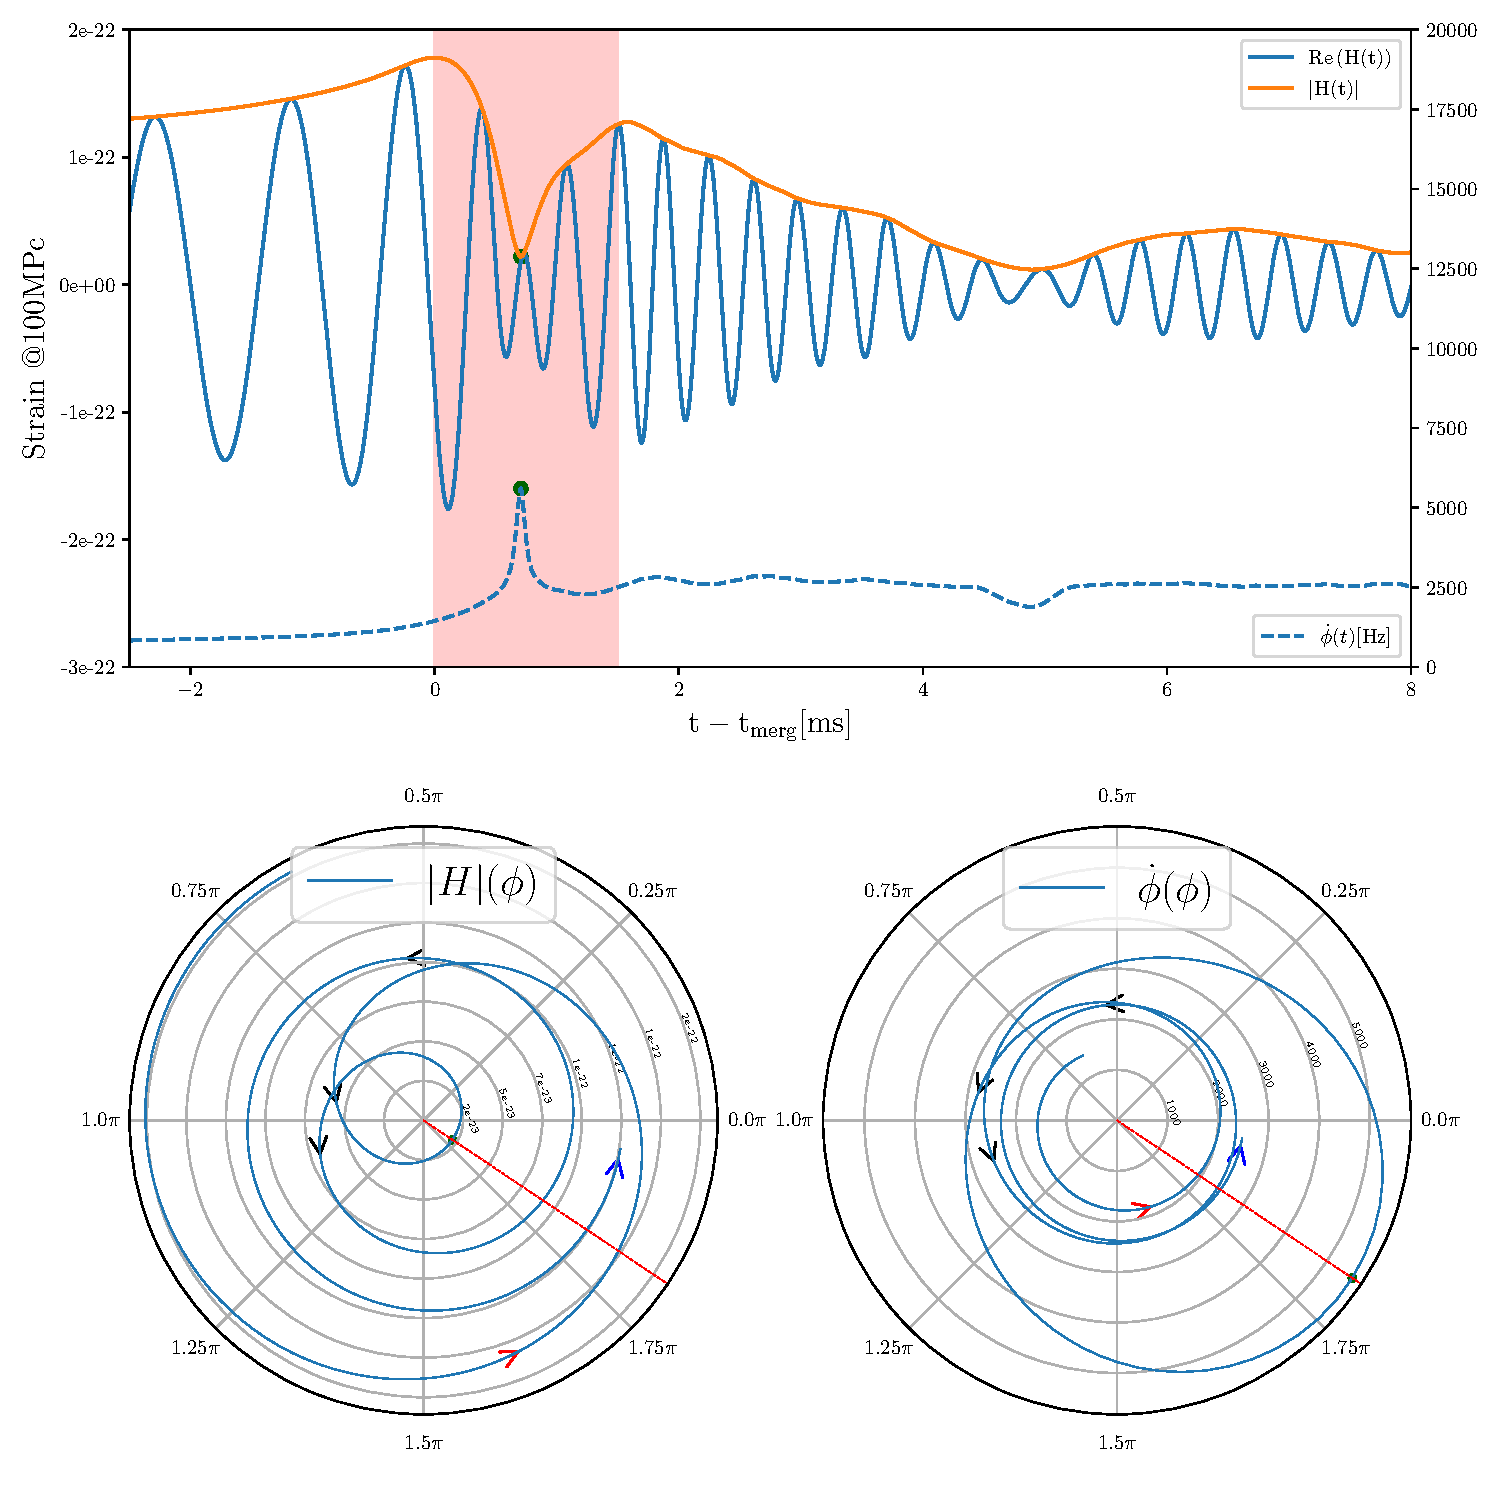
\includegraphics[width=0.7\textwidth, angle=0]{images/Data_analysis/results/postm_wf.pdf}
\end{center}
\captionsetup{width=0.8\textwidth}
\caption{The postmerger BNS signal}
\caption*{This figure contains the complex strain \ref{fvr} of a BNS waveform \cite{Dietrich:2018phi} with two local amplitude minima at 100MPc (top). The orbits of its amplitude $|H|(\phi)$ and phase velocity $\dot{\phi}(\phi)$ are represented in  the complex plane using polar coordinates (bottom). Only the samples of in the red region are represented to avoid seeing to many orbits.
Both polar plots contain 2 colored arrows to indicate time orientation. The red arrow marking earlier waveform samples, and the blue arrow marking later ones. Finally a constant red dashed line is used to mark the phase $\phi$ at which the amplitude minima and maximum phase velocity coincide.}
\label{fig:9} 
\end{figure}

\FloatBarrier

The smooth transition between late inspiral, merger and the postmerger phase of a BNS coalescense makes defining a starting point of a postmerger waveform a debatable subject. What is physically happening is a smooth transition from the time the atmospheres of the stars touch, and later the cores merge to produce the remnant. However, even thought there is not a single time sample that marks the beginning of the postmerger phase, this work will take the maximum amplitude of the $l=2$ $m=2$ mode as such. 

In order to define naturally a duration of the postmerger tail, a rectangular window function will be multiplied to every waveform to introduce a hard cut in between the maximum amplitude of the $l=2$ $m=2$ mode denoted as $t_{merg}$, and a threshold based duration defined as follows:

“$d_{postm}=$ the last time sample of the waveform with an amplitude above 5\% waveform’s maximum amplitude  ”

The inclusion of  such a threshold is required not to miscount portions of  waveforms that have a tail with negligible amplitude(see figure\ref{postm_cut} bottom panel)
Some other tapering windows could be used to make a postmerger signal that falls off smoothly on its edges. Even though tapering avoids spectral leakage effects when using DFTs, it will only make the duration definition more complicated. 

\begin{figure}[hbt!]
\begin{center}
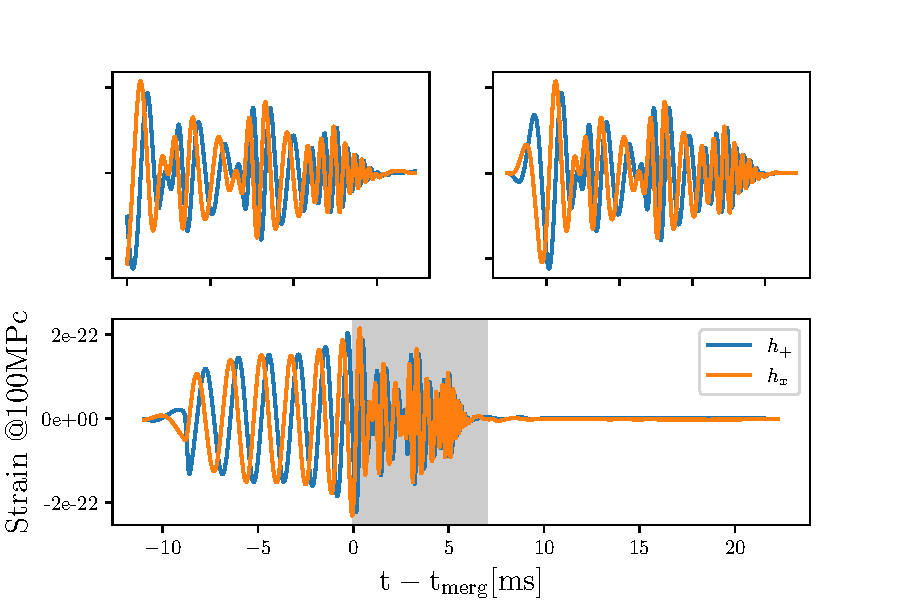
\includegraphics[width=\textwidth, angle=0]{{images/Data_analysis/results/d_postm.pdf}}
\captionsetup{width=0.8\textwidth}
\caption{The postmerger duration}
\caption*{This figure depicts two windowing options to extract the postmerger signal. The hard cutoff introduced by a rectangular window(upper right), which is contrasted with the case of a smooth tapering window like the Tukey one(upper left). The strain is taken from \cite{}.}
\end{center}
\label{postm_cut}
\end{figure}

\FloatBarrier


Existing sophisticated postmerger models \cite{Breschi:2019srl, Tsang:2019esi, Soultanis:2021oia, https://doi.org/10.48550/arxiv.2205.09112} are currently state-of-the-art research. For this reason, this thesis uses instead waveforms

After examining the BNS GW postmerger in the dataset mentioned in section \ref{NR}, we could observe that postmerger waveforms look very different depending on the input physics one considers. However,  we try making a rough classification, according to their length, number of amplitude minima and some other features that are easy to identify in this set of waveforms: 



\begin{itemize}
\item Equal mass systems ($q=1$) with low total gravitational mass ($\delta=\frac{M}{M_{TOV}}<1.6$). Such systems show only one deep amplitude minimum after merger followed by a tail of similar amplitude.

\item Systems with high mass ratio ($q>1.5$). Such systems show at least one loud signal cycle after merger, followed by a long low amplitude tail.

\item Spinning systems ($\chi_{eff}>0.2$). Such systems show several amplitude minima, and a tail with similar amplitude.

\item Systems with high total gravitational mass ($\delta=\frac{M}{M_{TOV}}>1.6$). Such systems have a short high frequency signal.

\item Highly eccentric systems ($e>0.4$). This systems may show several cycles before the first minimum, followed by a tail with similar amplitude.

\item Equal mass systems where viscous hydrodynamics is taken into account show a postmerger tail with stronger amplitude modulation.

\end{itemize}


\begin{figure}[hbt!]
\begin{center}
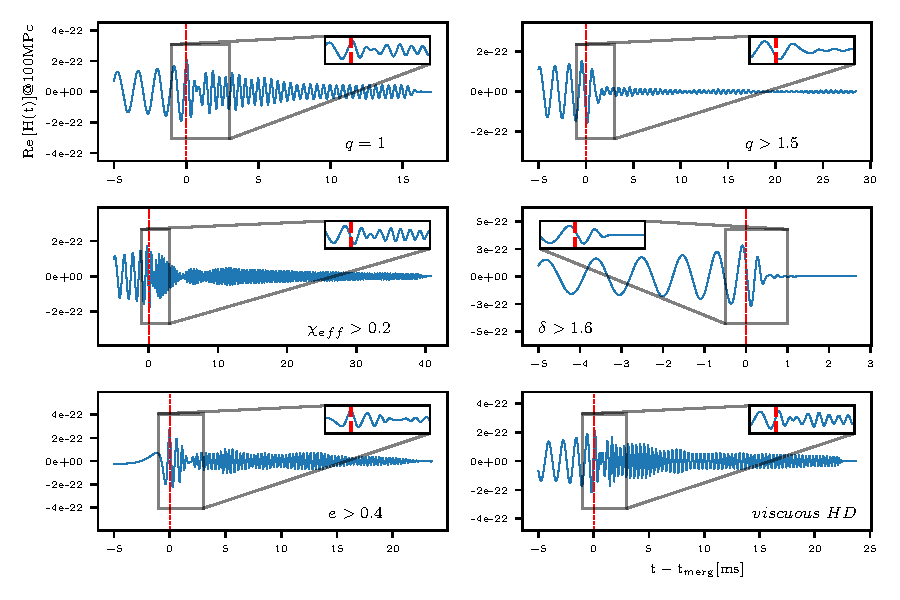
\includegraphics[width=\textwidth, angle=0]{images/Data_analysis/results/postm_wf_grid.pdf}
\captionsetup{width=0.8\textwidth}
\caption{BNS postmerger waveforms}
\caption*{Set of waveforms examples at 100MPc, the strain was obtained from \cite{}. It shows 6 different types of morphology present in a dataset of 220 waveforms. If the figure is read as a matrix, the plot 11 shows a equal mass systems($q=1$), the plot 12 a system with high mass ratio ($q>1.6$), the plot 21 a spinning system ($\chi_{_{eff}}>0.2$), the plot 22 a heavy systems ($\delta=\frac{M}{M_{TOV}}>1.6$), the plot 31 a highly eccentric systems ($e>0.4$) and the plot 32 system with equal masses with viscous hydrodynamics.}
\end{center}
\label{fig:10}
\end{figure}

\FloatBarrier 


One can use physical observables such as masses, and mass ratios along with gravitational wave properties in the time domain to examine whether there is any correlation between these physical parameters and the duration of the postmerger stage \ref{} in the dataset of 220 waveforms presented in the previous section. 

The following scatterplot shows that for waveforms in the catalog that were generated by BNS systems with a total mass greater than 1.6 times the maximum TOV mass, the gravitational waves of the postmerger stage last less than 5 milliseconds.

\begin{figure}[hbt!]
\begin{center}
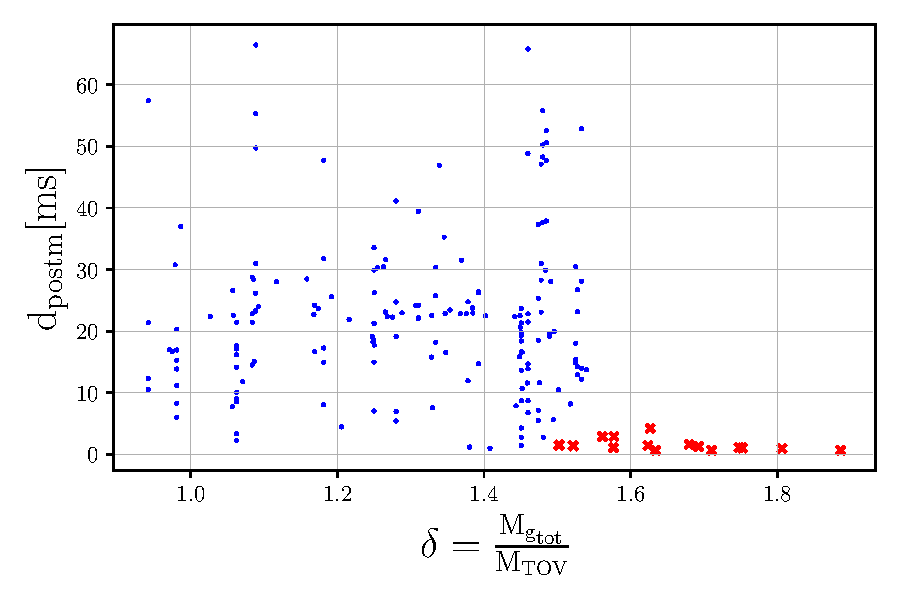
\includegraphics[width=0.7\textwidth, angle=0]{images/Data_analysis/results/res0.pdf}
\captionsetup{width=0.8\textwidth}
\caption{Can heavy systems have a long postmerger duration?}
\caption*{This scatterplot shows the relation of the postmerger BNS GW signal and the parameter $\delta$, which measures how heavy the system is with respect to the maximum TOV mass. It easily depicts that above some threshold mass, postmerger signals are very short \cite{Kashyap_2022}.}
\label{heavy systems}
\end{center}
\end{figure}


In addition, the few waveforms present in the catalog that have a mass ratio greater than 1.6 have a very small amplitude weighted duration, which is consistent with the high mass ratio example present in Figure \ref{} in which a postmerger stage is seen with a large amplitude just after the merger but which decays abruptly and continues with a low amplitude tail.


\begin{figure}[hbt!]
\begin{center}
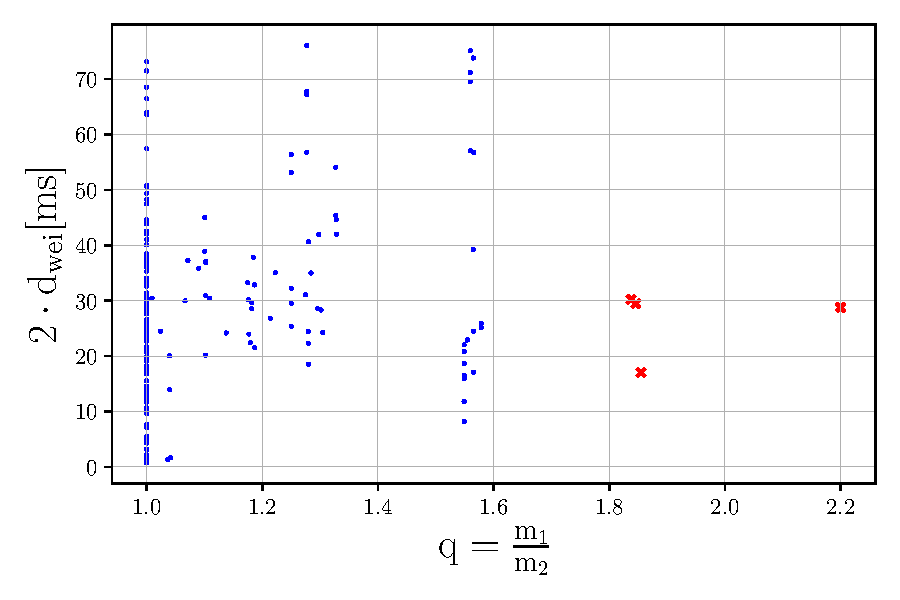
\includegraphics[width=0.7\textwidth, angle=0]{images/Data_analysis/results/Mr.pdf}
\captionsetup{width=0.8\textwidth}
\caption{The amplitude weighted duration of a high mass ratio waveform}
\caption*{This picture shows a possible influence of the high mass ratio (q>1.6) on waveforms with a particular morphology characterized by a  short amplitude weighted duration. The community has studied such a threshold in papers like \cite{Kolsch:2021lub}.}
\label{High mass ratio}
\end{center}
\end{figure}
\FloatBarrier


In addition, one can compare the quantities $d_{wei}$ \ref{} and $f_{wei}$ \ref{}, with the duration $d_{postm}$ and the most dominant frequency of the postmerger signal spectrum $f_2$. Note that the frequency $f_2$ was calculated by finding the location of the global maximum in the spectrum of each postmerger BNS signal. Such a comparison can be used to determine in which cases the $d_{wei}$ \ref{} and $f_{wei}$ \ref{} quantities match relatively well with the predefined $d_{postm}$ and $f_2$ quantities.

Note that from the two plots it can be concluded that both quantities match $d_{postm}$ and $f_2$ except for certain waveforms that deviate from the main correlation pattern. In the case of $d_{wei}$ the signals that deviate the most from the main straight line are highly eccentric simulations. Moreover, in the case of $f_{wei}$ the outliers are high mass ratio simulations.

\begin{figure}[hbt!]
\begin{center}
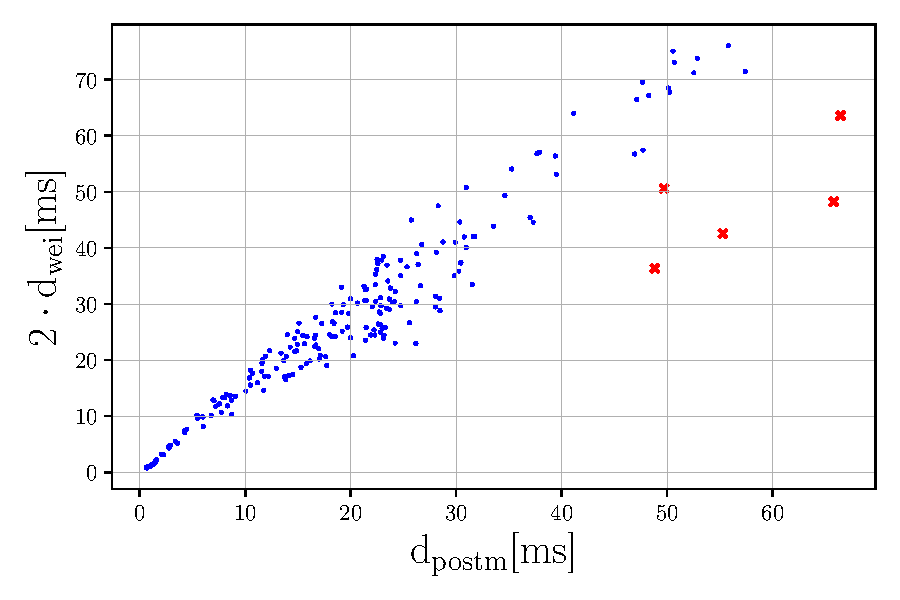
\includegraphics[width=0.7\textwidth, angle=0]{images/Data_analysis/results/res1.pdf}
\captionsetup{width=0.8\textwidth}
\caption{The postmerger amplitude weighted duration}
\caption*{This scatterplot compares the threshold-based duration $d_{postm}$ and the amplitude weighted one $d_{wei}$. Such a plot can tell how well an artificially defined threshold-based duration can reproduce the amplitude-weighted duration. Highly eccentric waveforms(red crosses) deviate the most from a straight line with a slope of 1, while the rest waveforms show a good agreement in both quantities.}
\label{duration measure}
\end{center}
\end{figure}


\begin{figure}[hbt!]
\begin{center}
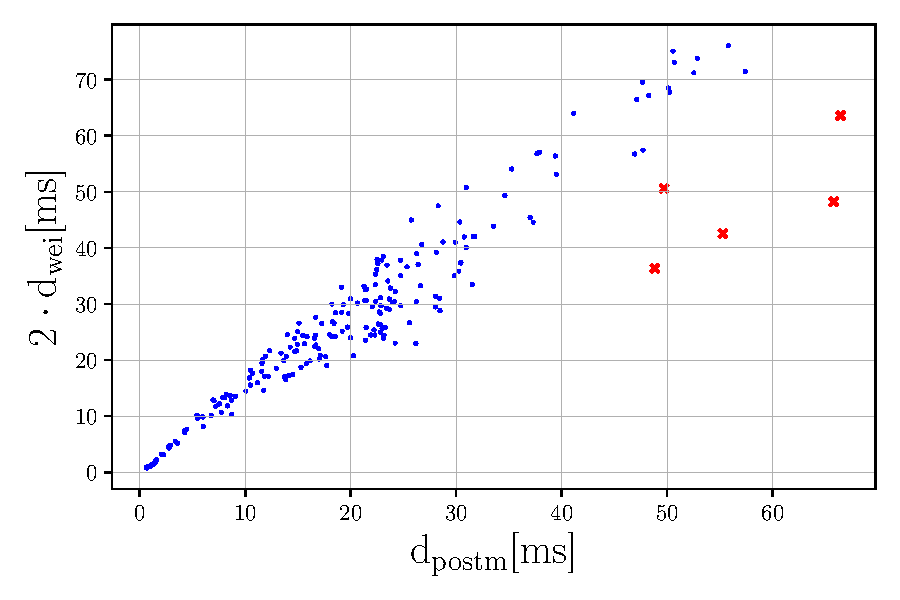
\includegraphics[width=0.7\textwidth, angle=0]{images/Data_analysis/results/res1.pdf}
\captionsetup{width=0.8\textwidth}
\caption{The postmerger amplitude weighted frequency}
\caption*{This scatterplot compares the threshold-based duration $d_{postm}$ and the amplitude weighted one $d_{wei}$. Such a plot can tell how well an artificially defined threshold-based duration can reproduce the amplitude-weighted duration. Highly eccentric waveforms(red crosses) deviate the most from a straight line with a slope of 1, while the rest waveforms show a good agreement in both quantities.}
\label{duration measure}
\end{center}
\end{figure}

\FloatBarrier







